% latexmk -pdflatex='xelatex %O %S' -pvc -pdf slides.tex
\documentclass{beamer}

\beamertemplatenavigationsymbolsempty

% für xelatex:
\usepackage{xltxtra}
\usepackage{unicode-math}

% literatur
\usepackage[backend=biber,style=alphabetic]{biblatex}

\addbibresource{../util/literature.bib}

\usepackage{../util/zariski}

\usepackage{csquotes}
\usepackage{cancel}
\usepackage{tabularx}
\usepackage{hyperref}
\usepackage{tikz}
\usetikzlibrary{cd,arrows,shapes,calc,through,backgrounds,matrix,trees,decorations.pathmorphing,positioning,automata}
\usepackage{graphicx}
\usepackage{color}

\usepackage{mathpartir}
\newcommand{\yields}{\vdash}
\newcommand{\cbar}{\, | \,}


% für tabellen
\usepackage{booktabs}

\title{Towards Synthetic Serre-Duality}
\date{May 22nd, 2025}

\begin{document}

\begin{frame}
  \titlepage
\end{frame}

\begin{frame}
  This and related work is and was done by:
  \begin{center}
    \begin{tabularx}{\textwidth}{XXX}
      Peter Arndt & Ulrik Buchholtz & Ingo Blechschmidt \\
      Felix Cherubini & Thierry Coquand & Fabian Endres \\
      Freek Geerligs & Jonas Höfer & Tim Lichtnau \\
      Hugo Moeneclaey & Marc N-W & Matthias Ritter \\
      Christian Sattler & Lukas Stoll & David Wärn \\
      Mark Williams & & 
    \end{tabularx}
  \end{center}
\end{frame}

\begin{frame}
  \vspace{1cm}
  \begin{center}
    \begin{tikzpicture} 
      [ 
      node distance=.8cm, 
      circled/.style={draw, ellipse, ultra thick, fill=blue!12},
      edge from parent/.style={very thick,draw=black,-latex},
      plaintext/.style={}
      ]

      \tikzstyle{level 1}=[sibling angle=81,level distance=4cm]

      \node[circled] (hott) {HoTT+Data+Axioms} [counterclockwise from=207]
      child { 
        node[circled] (grp) {$\infty$-Groupoids} 
        edge from parent [-latex] node (grp) 
        {
          \begin{tikzpicture}[scale=0.8, rotate=25]
            \draw[-, red, ultra thick] (0,0) to (1,1);
            \draw[-, red, ultra thick] (1,0) to (0,1);
          \end{tikzpicture}
        } 
      }
      child { node[matrix, circled, inner sep=0pt] (smgrp) 
        {
          \node[circled, minimum height=0.7cm, minimum width=3cm] (mfd) {Schemes};
          \node[below of=mfd, text width=3cm,
          node distance=0.9cm] 
          {``Constructive Zariski-sheaves''}; \\
        }
      }
      ;
    \end{tikzpicture}
  \end{center}
  \vspace{1cm}
  {\footnotesize * Schemes = quasi-compact, quasi-separated schemes of finite presentation}
\end{frame}

\begin{frame}
    
  Morphisms of schemes should be locally polynomial. \\
  \pause
  $\Rightarrow$ Correspondence between affine schemes and algebra: \\
  \pause
  \begin{center}
    \begin{tabular}{ll}
      Affine Schemes & $\to$ $R$-algebras \\
      $V$ & $\mapsto R^V$
    \end{tabular}
  \end{center}
  \pause
  One classical way to turn this into an (anti) equivalence of categories,
  is to give affine schemes a lot more structure than just subsets of $R^n$.
\end{frame}

\begin{frame}
  \frametitle{Now: \textbf{Synthetic} Algebraic Geometry}
  \pause
  $R$ is a given commutative ring from now on. \\
  \vspace{0.4cm}
  \pause

  $V\coloneq \{(x,y):R^2\mid x^2+y^2=1 \}$ \\

  \pause
  Adding equations like $0=0$, $x(x^2+y^2)=x$ does not change the type $V$. \\
  \pause
  $V$ is determined by the $R$-algebra $A\coloneq R[X,Y]/(X^2+Y^2-1)$.
  \pause
  We can recover it: $V=\Hom_{\Alg{R}}(A,R)$. \\
  \vspace{0.4cm}
  \pause
  \begin{definition}
    \begin{enumerate}[(i)]
    \item An $R$-algebra is finitely presented (fp) if it is merely $R[X_1,\dots,X_n]/(P_1,\dots,P_l)$.
    \item $\Spec(A)\coloneq \Hom_{\Alg{R}}(A,R)$ is the \emph{spectrum} of an fp $R$-algebra $A$.
    \item Any $X$ such that there is an $A$ with $X=\Spec(A)$ is called \emph{affine scheme}.
    \end{enumerate}
  \end{definition}
\end{frame}

\begin{frame}
  \frametitle{The 3 Axioms of SAG}
    \textbf{Axiom (Duality):}
    The map
    \begin{align*}
      A \to R^{\Spec A} \\
      a\mapsto (\varphi\mapsto \varphi(a))
    \end{align*}
    is an equivalence
    for any finitely presented $R$-algebra $A$. \\
  \pause
  \vspace{1.5mm}
  \textbf{Axiom (Locality):} The ring $R$ is local.

  \vspace{1.5mm}
  \textbf{Axiom (Zariski-local choice):}\\
  For every surjective $\pi$, there merely exist local sections $s_i$
  \[ \begin{tikzcd}[ampersand replacement=\&, column sep=small]
    \& E \ar[d, two heads, "\pi"] \\
    D(f_i) \ar[r, hook] \ar[ur, bend left, dashed, "s_i"] \& \Spec(A)
  \end{tikzcd} \]
  with $f_1, \dots, f_n : A$ such that $(f_1,\dots,f_n)=(1)$.
\end{frame}

{ % all template changes are local to this group.
    \setbeamertemplate{navigation symbols}{}
    \begin{frame}<article:0>[plain]
        \begin{tikzpicture}[remember picture,overlay]
            \node[at=(current page.center)] {
                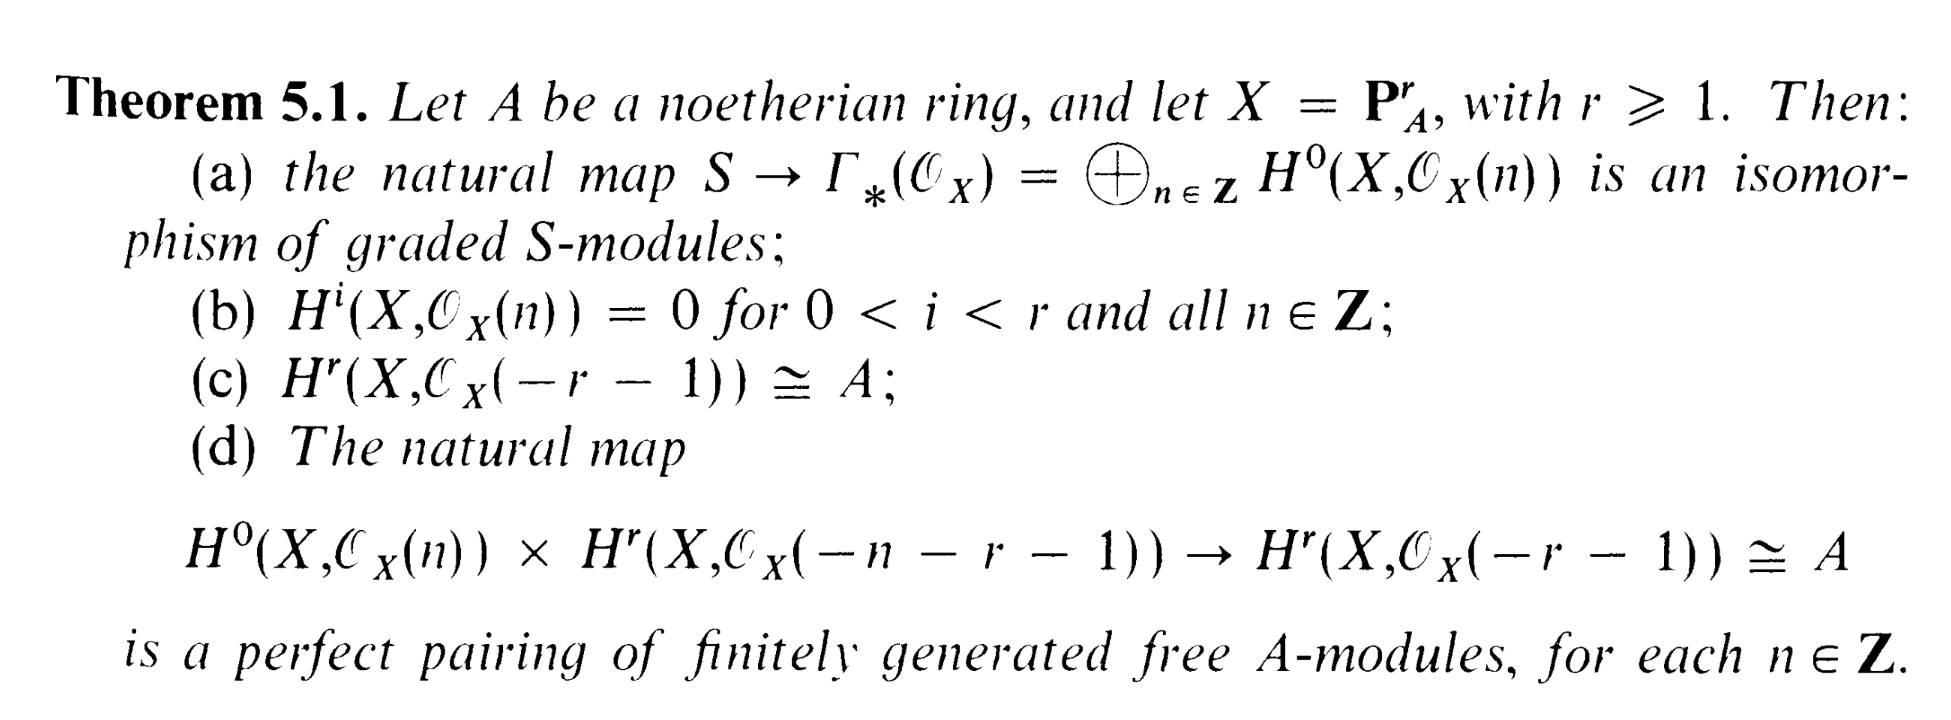
\includegraphics[keepaspectratio,
                                 width=\paperwidth,
                                 height=\paperheight]{hartshorne2.png}
            };
        \end{tikzpicture}
     \end{frame}
}

{ % all template changes are local to this group.
    \setbeamertemplate{navigation symbols}{}
    \begin{frame}<article:0>[plain]
        \begin{tikzpicture}[remember picture,overlay]
            \node[at=(current page.center)] {
                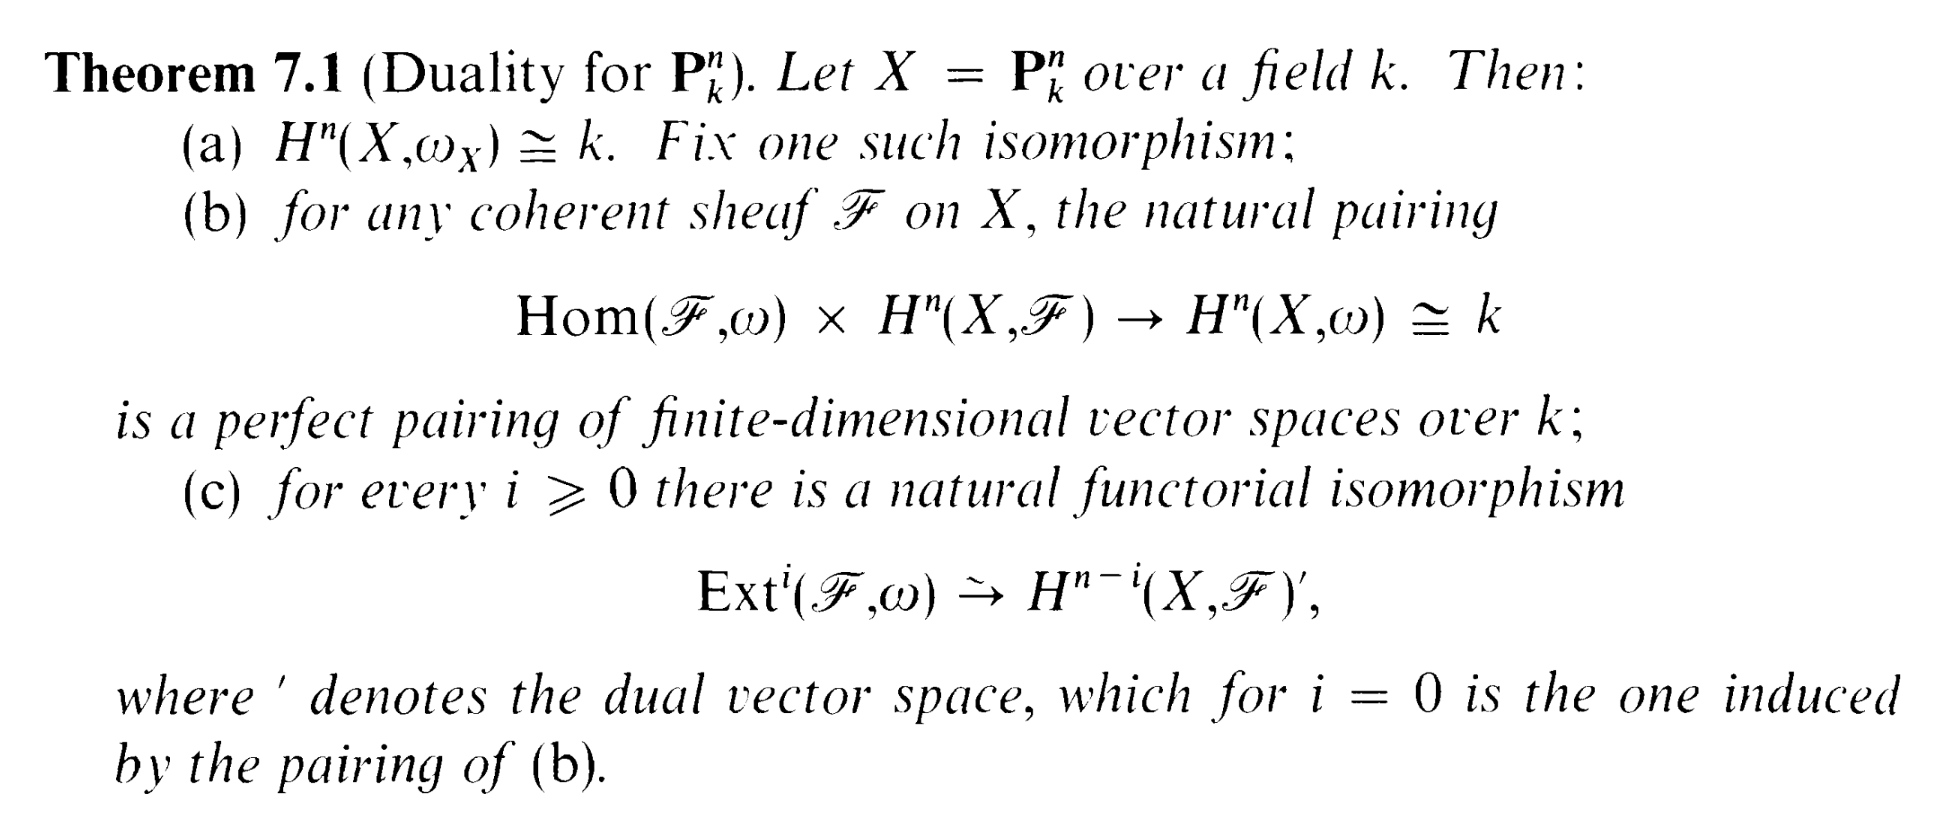
\includegraphics[keepaspectratio,
                                 width=\paperwidth,
                                 height=\paperheight]{hartshorne1.png}
            };
        \end{tikzpicture}
     \end{frame}
}


\begin{frame}
  \frametitle{Selected Results and Definitions (SAG)}
  A type $X$ is a \textbf{scheme} if
  there exist open $U_1, \dots, U_n \subseteq X$
  such that $X = \bigcup_i U_i$
  and every $U_i$ is an affine scheme. \\
  \vspace{5mm}
  \pause
  \textbf{Morphisms} of schemes are just maps between types.
  
  \pause
  \vspace{5mm}
  \textbf{Example.}
  \emph{Projective $n$-space}:
  \begin{align*}
    \bP^n
    &\coloneq \{x : R^{n+1}\mid x\neq 0\}/\approx\text{ where $(x\approx y)\coloneq \exists \lambda:R. \lambda x= y$}\} \\
    &= \{\,\text{submodules $L\subseteq R^{n+1}$ such that $\|L=R^1\|$}\,\}
  \end{align*}
  is a scheme, since
  \[
    U_i([x]) \coloneq \text{($x_i$ is invertible)}
  \]
  is an open affine cover.
\end{frame}

\begin{frame}
  \frametitle{Selected Results and Definitions (SAG)}
  Schemes are closed under $\Sigma$-types and identity types. \\
  \pause
  \vspace{1cm}
  \emph{Classical equivalent}: Schemes are closed under pullbacks. \\
  \pause
  \vspace{1cm}
  SAG statement is more general. \\
  \vspace{1cm}
\end{frame}

\begin{frame}
  \frametitle{Selected Results and Definitions (SAG)}
  \vspace{0.25cm}
  For $A : X \to \mathrm{Ab}$, define \emph{cohomology} as:
  \[ H^n(X, A) :\equiv \Big\| \prod_{x:X}K(A_x,n) \Big\|_{\mathrm{set}} \]
  
  \pause
  Good because:
  \begin{itemize}
  \item $\prod$-type.
  \item $\|\_\|_{\mathrm{set}}$ is a modality.
  \item Homotopy group: $H^n(X,A)=\pi_{k}(\prod_{x:X}K(A,n+k))$.
  \end{itemize}

  \pause
  Non-trivial for $X:\mathrm{Set}$ because:

  $X=$ Pushout of sets $U\leftarrow Y\to V$, \\
  Then a ``cohomology class'' $X\to K(A,1)$ is given by:
  \begin{itemize}
  \item Maps $f:U\to K(A,1)$, $g:V\to K(A,1)$.
  \item And $h:(x:Y)\to f(x)=g(x)$, which is essentially a map $Y\to A$,
    if $U$ and $V$ do not have higher cohomology...
  \end{itemize}
\end{frame}

\begin{frame}
  \frametitle{Selected Results and Definitions (SAG)}

  Let
  \[ \mathrm{Lines} \coloneq \sum_{L : R\text{-Mod}} \lVert L = R^1 \rVert \]

  \pause
  \vspace{5mm}
  The \emph{Picard group} of $X$ is
  \[ \mathrm{Pic}(X) \coloneq \lVert X \to \mathrm{Lines} \rVert_{\text{set}} \rlap{.}\]
  
  \pause
  We have $\mathrm{Pic}(\mathbb P^n)=\mathbb Z$. \\
  \pause
  And the more general: $(\mathbb P^n \to \mathrm{Lines}) = \mathbb Z \times \mathrm{Lines}$. \\
\end{frame}

\begin{frame}
  \frametitle{Concluding remarks on SAG and SSD}
  \begin{enumerate}[(1)]
  \item Models in constructive meta-theory.
  \item Unclear how much of the classical theory is reproducible in this way.
  \item Type theory sometimes leads to a nicer formulation of results.
  \item Far away from mainstream practice.
  \item Might admit significantly shorter formalization. 
  \end{enumerate}
\end{frame}

\end{document}
